\documentclass[tikz,border=10pt]{standalone}
\usepackage{amsmath,amssymb}
\usetikzlibrary{arrows.meta}

% 同色系蓝阶渐变
\definecolor{cZero}{RGB}{6, 78, 59}     % 0阶：墨绿
\definecolor{cOne}{RGB}{4, 120, 87}     % 1阶：深翠绿
\definecolor{cTwo}{RGB}{5, 150, 105}    % 2阶：翡翠绿
\definecolor{cDots}{RGB}{156, 163, 160} % 省略层：石板灰绿
\definecolor{cN}{RGB}{16, 185, 129}     % n阶：翠绿
\definecolor{cFinal}{RGB}{52, 211, 153} % n+1阶：亮薄荷绿
\definecolor{divCol}{RGB}{209, 213, 219}% 分割线：浅灰

\begin{document}
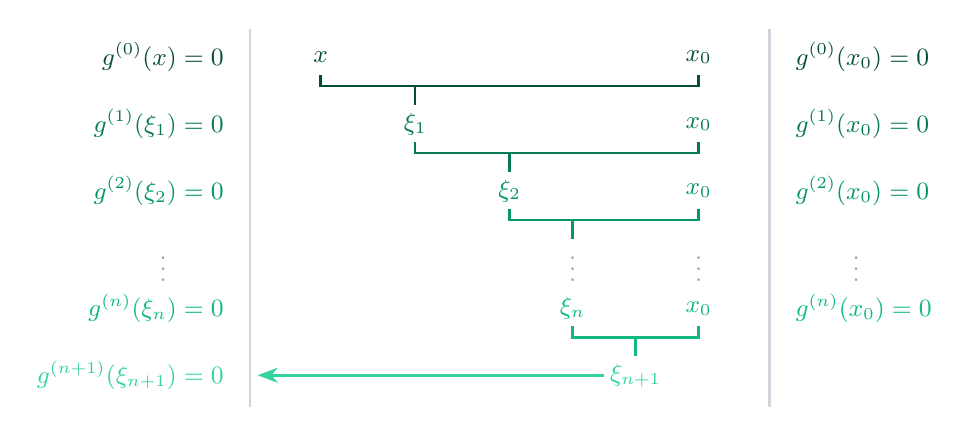
\begin{tikzpicture}[
    thick,
    >=Stealth,
    font=\small,
    bracket/.style={line width=0.85pt}
]

    % ================= 左右两侧纵向分割线 =================
    \draw[divCol, line width=0.8pt] (-3.3, 0.45) -- (-3.3, -4.35);
    \draw[divCol, line width=0.8pt] ( 3.3, 0.45) -- ( 3.3, -4.35);

    % ================= 0 层: [x, x_0] (文字 y = 0.09) =================
    \node[anchor=east, text=cZero] at (-3.5, 0.09) {$g^{(0)}(x) = 0$};
    \node[anchor=west, text=cZero] at ( 3.5, 0.09) {$g^{(0)}(x_0) = 0$};
    \node[text=cZero] at (-2.4, 0.09) {$x$};
    \node[text=cZero] at ( 2.4, 0.09) {$x_0$};
    \draw[cZero, bracket] 
        (-2.4, -0.14) -- (-2.4, -0.28) -- (2.4, -0.28) -- (2.4, -0.14);
    \draw[cZero, bracket] 
        (-1.2, -0.28) -- (-1.2, -0.52);

    % ================= 1 层: [\xi_1, x_0] (文字 y = -0.76) =================
    \node[anchor=east, text=cOne] at (-3.5, -0.76) {$g^{(1)}(\xi_1) = 0$};
    \node[anchor=west, text=cOne] at ( 3.5, -0.76) {$g^{(1)}(x_0) = 0$};
    \node[text=cOne] at (-1.2, -0.76) {$\xi_1$};
    \node[text=cOne] at ( 2.4, -0.76) {$x_0$};
    \draw[cOne, bracket] 
        (-1.2, -0.99) -- (-1.2, -1.13) -- (2.4, -1.13) -- (2.4, -0.99);
    \draw[cOne, bracket] 
        (0.0, -1.13) -- (0.0, -1.37);

    % ================= 2 层: [\xi_2, x_0] (文字 y = -1.61) =================
    \node[anchor=east, text=cTwo] at (-3.5, -1.61) {$g^{(2)}(\xi_2) = 0$};
    \node[anchor=west, text=cTwo] at ( 3.5, -1.61) {$g^{(2)}(x_0) = 0$};
    \node[text=cTwo] at (0.0, -1.61) {$\xi_2$};
    \node[text=cTwo] at (2.4, -1.61) {$x_0$};
    \draw[cTwo, bracket] 
        (0.0, -1.84) -- (0.0, -1.98) -- (2.4, -1.98) -- (2.4, -1.84);
    \draw[cTwo, bracket] 
        (0.8, -1.98) -- (0.8, -2.22);

    % ================= 省略号层 (y = -2.60，适度上收保持视觉对称) =================
    \node[text=cDots] at (-4.4, -2.50) {$\vdots$};
    \node[text=cDots] at ( 0.8, -2.50) {$\vdots$};
    \node[text=cDots] at ( 2.4, -2.50) {$\vdots$};
    \node[text=cDots] at ( 4.4, -2.50) {$\vdots$};

    % ================= n 层: [\xi_n, x_0] (文字 y = -3.10) =================
    \node[anchor=east, text=cN] at (-3.5, -3.10) {$g^{(n)}(\xi_n) = 0$};
    \node[anchor=west, text=cN] at ( 3.5, -3.10) {$g^{(n)}(x_0) = 0$};
    \node[text=cN] at (0.8, -3.10) {$\xi_n$};
    \node[text=cN] at (2.4, -3.10) {$x_0$};
    \draw[cN, bracket] 
        (0.8, -3.33) -- (0.8, -3.47) -- (2.4, -3.47) -- (2.4, -3.33);
    \draw[cN, bracket] 
        (1.6, -3.47) -- (1.6, -3.71);

    % ================= n+1 层: \xi_{n+1} 与最终推导 (文字 y = -3.95) =================
    \node[anchor=east, text=cFinal] at (-3.5, -3.95) {$g^{(n+1)}(\xi_{n+1}) = 0$};
    \node[text=cFinal] at (1.6, -3.95) {$\xi_{n+1}$};
    \draw[->, cFinal, line width=0.95pt] (1.2, -3.95) -- (-3.2, -3.95);

\end{tikzpicture}
\end{document}